\documentclass{article}

\begin{document}

\setlength{\parindent}{6ex}

\indent

Object detection is a concept of computer vision in which trained models 
detect objects with their category and location in given images or videos. 
As you can see in figure \ref{fig:bicycle1}, object detection is both 
classifying and localizing the object instances in given images. Also, the 
parts of the given image that contain no object is called background.

\begin{figure}
    \centering
    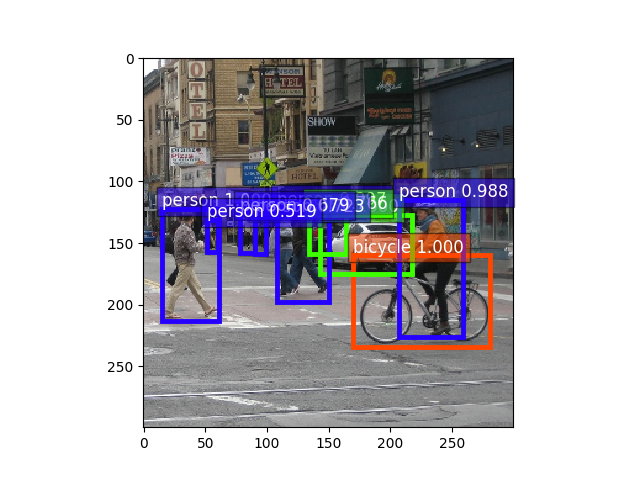
\includegraphics[width=\textwidth]{bicycle}
    \caption{Example of Object Detection}
    \label{fig:bicycle1}
\end{figure}
\end{document}